

\tikzset{every picture/.style={line width=0.75pt}} %set default line width to 0.75pt        

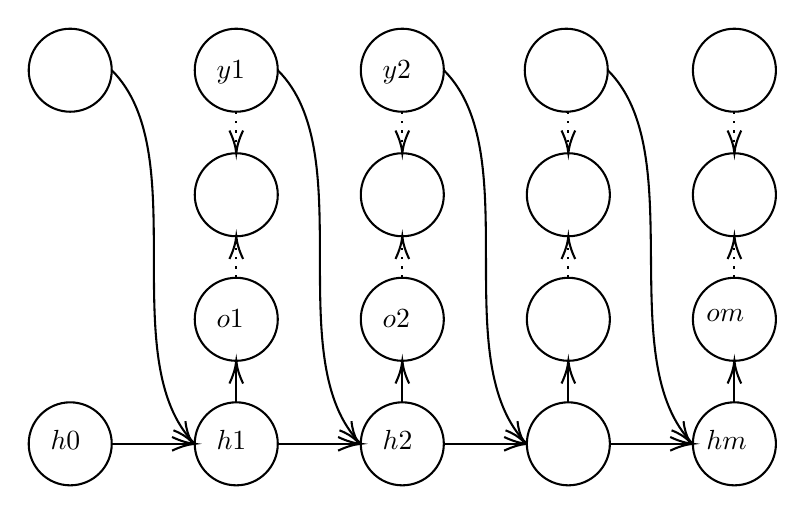
\begin{tikzpicture}[x=0.75pt,y=0.75pt,yscale=-1,xscale=1]
%uncomment if require: \path (0,300); %set diagram left start at 0, and has height of 300

%Straight Lines [id:da23603443129614066] 
\draw    (220,230) -- (258,230) ;
\draw [shift={(260,230)}, rotate = 180] [color={rgb, 255:red, 0; green, 0; blue, 0 }  ][line width=0.75]    (10.93,-3.29) .. controls (6.95,-1.4) and (3.31,-0.3) .. (0,0) .. controls (3.31,0.3) and (6.95,1.4) .. (10.93,3.29)   ;
%Curve Lines [id:da06456839015717697] 
\draw    (220,50) .. controls (260.2,89.92) and (220.6,190.32) .. (260,230) ;
\draw   (255.51,219.09) .. controls (255.87,222.89) and (256.88,226.21) .. (258.53,229.03) .. controls (256.24,226.7) and (253.3,224.85) .. (249.73,223.5) ;
%Shape: Circle [id:dp8656589914443553] 
\draw   (100,170) .. controls (100,158.95) and (108.95,150) .. (120,150) .. controls (131.05,150) and (140,158.95) .. (140,170) .. controls (140,181.05) and (131.05,190) .. (120,190) .. controls (108.95,190) and (100,181.05) .. (100,170) -- cycle ;
%Shape: Circle [id:dp06290087538404654] 
\draw   (180,170) .. controls (180,158.95) and (188.95,150) .. (200,150) .. controls (211.05,150) and (220,158.95) .. (220,170) .. controls (220,181.05) and (211.05,190) .. (200,190) .. controls (188.95,190) and (180,181.05) .. (180,170) -- cycle ;
%Shape: Circle [id:dp7703553130285721] 
\draw   (340,170) .. controls (340,158.95) and (348.95,150) .. (360,150) .. controls (371.05,150) and (380,158.95) .. (380,170) .. controls (380,181.05) and (371.05,190) .. (360,190) .. controls (348.95,190) and (340,181.05) .. (340,170) -- cycle ;
%Shape: Circle [id:dp46492369967762426] 
\draw   (100,230) .. controls (100,218.95) and (108.95,210) .. (120,210) .. controls (131.05,210) and (140,218.95) .. (140,230) .. controls (140,241.05) and (131.05,250) .. (120,250) .. controls (108.95,250) and (100,241.05) .. (100,230) -- cycle ;
%Shape: Circle [id:dp8326413265399102] 
\draw   (180,230) .. controls (180,218.95) and (188.95,210) .. (200,210) .. controls (211.05,210) and (220,218.95) .. (220,230) .. controls (220,241.05) and (211.05,250) .. (200,250) .. controls (188.95,250) and (180,241.05) .. (180,230) -- cycle ;
%Shape: Circle [id:dp5294418510367744] 
\draw  [fill={rgb, 255:red, 255; green, 255; blue, 255 }  ,fill opacity=1 ] (340,230) .. controls (340,218.95) and (348.95,210) .. (360,210) .. controls (371.05,210) and (380,218.95) .. (380,230) .. controls (380,241.05) and (371.05,250) .. (360,250) .. controls (348.95,250) and (340,241.05) .. (340,230) -- cycle ;
%Shape: Circle [id:dp42103973093131075] 
\draw   (100,110) .. controls (100,98.95) and (108.95,90) .. (120,90) .. controls (131.05,90) and (140,98.95) .. (140,110) .. controls (140,121.05) and (131.05,130) .. (120,130) .. controls (108.95,130) and (100,121.05) .. (100,110) -- cycle ;
%Shape: Circle [id:dp936509666827531] 
\draw   (180,110) .. controls (180,98.95) and (188.95,90) .. (200,90) .. controls (211.05,90) and (220,98.95) .. (220,110) .. controls (220,121.05) and (211.05,130) .. (200,130) .. controls (188.95,130) and (180,121.05) .. (180,110) -- cycle ;
%Shape: Circle [id:dp5718122823533516] 
\draw   (340,110) .. controls (340,98.95) and (348.95,90) .. (360,90) .. controls (371.05,90) and (380,98.95) .. (380,110) .. controls (380,121.05) and (371.05,130) .. (360,130) .. controls (348.95,130) and (340,121.05) .. (340,110) -- cycle ;
%Shape: Circle [id:dp6301703620557764] 
\draw   (20,50) .. controls (20,38.95) and (28.95,30) .. (40,30) .. controls (51.05,30) and (60,38.95) .. (60,50) .. controls (60,61.05) and (51.05,70) .. (40,70) .. controls (28.95,70) and (20,61.05) .. (20,50) -- cycle ;
%Shape: Circle [id:dp6512803525821871] 
\draw   (100,50) .. controls (100,38.95) and (108.95,30) .. (120,30) .. controls (131.05,30) and (140,38.95) .. (140,50) .. controls (140,61.05) and (131.05,70) .. (120,70) .. controls (108.95,70) and (100,61.05) .. (100,50) -- cycle ;
%Shape: Circle [id:dp3497652254930159] 
\draw   (180,50) .. controls (180,38.95) and (188.95,30) .. (200,30) .. controls (211.05,30) and (220,38.95) .. (220,50) .. controls (220,61.05) and (211.05,70) .. (200,70) .. controls (188.95,70) and (180,61.05) .. (180,50) -- cycle ;
%Shape: Circle [id:dp2184847180228391] 
\draw   (20,230) .. controls (20,218.95) and (28.95,210) .. (40,210) .. controls (51.05,210) and (60,218.95) .. (60,230) .. controls (60,241.05) and (51.05,250) .. (40,250) .. controls (28.95,250) and (20,241.05) .. (20,230) -- cycle ;
%Shape: Circle [id:dp2975524043148017] 
\draw   (340,50) .. controls (340,38.95) and (348.95,30) .. (360,30) .. controls (371.05,30) and (380,38.95) .. (380,50) .. controls (380,61.05) and (371.05,70) .. (360,70) .. controls (348.95,70) and (340,61.05) .. (340,50) -- cycle ;
%Curve Lines [id:da9201167463907463] 
\draw    (60,50) .. controls (100.2,89.92) and (60.6,190.32) .. (100,230) ;
\draw   (95.51,219.09) .. controls (95.87,222.89) and (96.88,226.21) .. (98.53,229.03) .. controls (96.24,226.7) and (93.3,224.85) .. (89.73,223.5) ;
%Curve Lines [id:da49848787514665216] 
\draw    (140,50) .. controls (180.2,89.92) and (140.6,190.32) .. (180,230) ;
%Straight Lines [id:da821586298210278] 
\draw    (60,230) -- (98,230) ;
\draw [shift={(100,230)}, rotate = 180] [color={rgb, 255:red, 0; green, 0; blue, 0 }  ][line width=0.75]    (10.93,-3.29) .. controls (6.95,-1.4) and (3.31,-0.3) .. (0,0) .. controls (3.31,0.3) and (6.95,1.4) .. (10.93,3.29)   ;
%Straight Lines [id:da3929180892527673] 
\draw    (140,230) -- (178,230) ;
\draw [shift={(180,230)}, rotate = 180] [color={rgb, 255:red, 0; green, 0; blue, 0 }  ][line width=0.75]    (10.93,-3.29) .. controls (6.95,-1.4) and (3.31,-0.3) .. (0,0) .. controls (3.31,0.3) and (6.95,1.4) .. (10.93,3.29)   ;
%Straight Lines [id:da48950294540297135] 
\draw    (120,210) -- (120,192) ;
\draw [shift={(120,190)}, rotate = 450] [color={rgb, 255:red, 0; green, 0; blue, 0 }  ][line width=0.75]    (10.93,-3.29) .. controls (6.95,-1.4) and (3.31,-0.3) .. (0,0) .. controls (3.31,0.3) and (6.95,1.4) .. (10.93,3.29)   ;
%Straight Lines [id:da3700514576696854] 
\draw    (200,210) -- (200,192) ;
\draw [shift={(200,190)}, rotate = 450] [color={rgb, 255:red, 0; green, 0; blue, 0 }  ][line width=0.75]    (10.93,-3.29) .. controls (6.95,-1.4) and (3.31,-0.3) .. (0,0) .. controls (3.31,0.3) and (6.95,1.4) .. (10.93,3.29)   ;
%Straight Lines [id:da9053727006348504] 
\draw    (360,210) -- (360,192) ;
\draw [shift={(360,190)}, rotate = 450] [color={rgb, 255:red, 0; green, 0; blue, 0 }  ][line width=0.75]    (10.93,-3.29) .. controls (6.95,-1.4) and (3.31,-0.3) .. (0,0) .. controls (3.31,0.3) and (6.95,1.4) .. (10.93,3.29)   ;
%Straight Lines [id:da32485535303931923] 
\draw  [dash pattern={on 0.84pt off 2.51pt}]  (120,150) -- (120,132) ;
\draw [shift={(120,130)}, rotate = 450] [color={rgb, 255:red, 0; green, 0; blue, 0 }  ][line width=0.75]    (10.93,-3.29) .. controls (6.95,-1.4) and (3.31,-0.3) .. (0,0) .. controls (3.31,0.3) and (6.95,1.4) .. (10.93,3.29)   ;
%Straight Lines [id:da264284637761111] 
\draw  [dash pattern={on 0.84pt off 2.51pt}]  (200,150) -- (200,132) ;
\draw [shift={(200,130)}, rotate = 450] [color={rgb, 255:red, 0; green, 0; blue, 0 }  ][line width=0.75]    (10.93,-3.29) .. controls (6.95,-1.4) and (3.31,-0.3) .. (0,0) .. controls (3.31,0.3) and (6.95,1.4) .. (10.93,3.29)   ;
%Straight Lines [id:da24685635403217576] 
\draw  [dash pattern={on 0.84pt off 2.51pt}]  (360,150) -- (360,132) ;
\draw [shift={(360,130)}, rotate = 450] [color={rgb, 255:red, 0; green, 0; blue, 0 }  ][line width=0.75]    (10.93,-3.29) .. controls (6.95,-1.4) and (3.31,-0.3) .. (0,0) .. controls (3.31,0.3) and (6.95,1.4) .. (10.93,3.29)   ;
%Straight Lines [id:da8058559050356451] 
\draw  [dash pattern={on 0.84pt off 2.51pt}]  (120,70) -- (120,88) ;
\draw [shift={(120,90)}, rotate = 270] [color={rgb, 255:red, 0; green, 0; blue, 0 }  ][line width=0.75]    (10.93,-3.29) .. controls (6.95,-1.4) and (3.31,-0.3) .. (0,0) .. controls (3.31,0.3) and (6.95,1.4) .. (10.93,3.29)   ;
%Straight Lines [id:da03130540180118557] 
\draw  [dash pattern={on 0.84pt off 2.51pt}]  (200,70) -- (200,88) ;
\draw [shift={(200,90)}, rotate = 270] [color={rgb, 255:red, 0; green, 0; blue, 0 }  ][line width=0.75]    (10.93,-3.29) .. controls (6.95,-1.4) and (3.31,-0.3) .. (0,0) .. controls (3.31,0.3) and (6.95,1.4) .. (10.93,3.29)   ;
%Straight Lines [id:da6029515695196923] 
\draw  [dash pattern={on 0.84pt off 2.51pt}]  (360,70) -- (360,88) ;
\draw [shift={(360,90)}, rotate = 270] [color={rgb, 255:red, 0; green, 0; blue, 0 }  ][line width=0.75]    (10.93,-3.29) .. controls (6.95,-1.4) and (3.31,-0.3) .. (0,0) .. controls (3.31,0.3) and (6.95,1.4) .. (10.93,3.29)   ;
\draw   (175.51,219.09) .. controls (175.87,222.89) and (176.88,226.21) .. (178.53,229.03) .. controls (176.24,226.7) and (173.3,224.85) .. (169.73,223.5) ;
%Shape: Circle [id:dp14354017998827717] 
\draw  [color={rgb, 255:red, 0; green, 0; blue, 0 }  ,draw opacity=1 ][fill={rgb, 255:red, 255; green, 255; blue, 255 }  ,fill opacity=1 ] (260,230) .. controls (260,218.95) and (268.95,210) .. (280,210) .. controls (291.05,210) and (300,218.95) .. (300,230) .. controls (300,241.05) and (291.05,250) .. (280,250) .. controls (268.95,250) and (260,241.05) .. (260,230) -- cycle ;
%Shape: Circle [id:dp1325142417799936] 
\draw  [color={rgb, 255:red, 0; green, 0; blue, 0 }  ,draw opacity=1 ][fill={rgb, 255:red, 255; green, 255; blue, 255 }  ,fill opacity=1 ] (260,170) .. controls (260,158.95) and (268.95,150) .. (280,150) .. controls (291.05,150) and (300,158.95) .. (300,170) .. controls (300,181.05) and (291.05,190) .. (280,190) .. controls (268.95,190) and (260,181.05) .. (260,170) -- cycle ;
%Shape: Circle [id:dp14659583436002066] 
\draw  [color={rgb, 255:red, 0; green, 0; blue, 0 }  ,draw opacity=1 ][fill={rgb, 255:red, 255; green, 255; blue, 255 }  ,fill opacity=1 ] (260,110) .. controls (260,98.95) and (268.95,90) .. (280,90) .. controls (291.05,90) and (300,98.95) .. (300,110) .. controls (300,121.05) and (291.05,130) .. (280,130) .. controls (268.95,130) and (260,121.05) .. (260,110) -- cycle ;
%Shape: Circle [id:dp21508491391490026] 
\draw  [color={rgb, 255:red, 0; green, 0; blue, 0 }  ,draw opacity=1 ][fill={rgb, 255:red, 255; green, 255; blue, 255 }  ,fill opacity=1 ] (259,50) .. controls (259,38.95) and (267.95,30) .. (279,30) .. controls (290.05,30) and (299,38.95) .. (299,50) .. controls (299,61.05) and (290.05,70) .. (279,70) .. controls (267.95,70) and (259,61.05) .. (259,50) -- cycle ;
%Straight Lines [id:da6354968350696126] 
\draw    (280,210) -- (280,192) ;
\draw [shift={(280,190)}, rotate = 450] [color={rgb, 255:red, 0; green, 0; blue, 0 }  ][line width=0.75]    (10.93,-3.29) .. controls (6.95,-1.4) and (3.31,-0.3) .. (0,0) .. controls (3.31,0.3) and (6.95,1.4) .. (10.93,3.29)   ;
%Straight Lines [id:da44472942046558095] 
\draw  [dash pattern={on 0.84pt off 2.51pt}]  (280,150) -- (280,132) ;
\draw [shift={(280,130)}, rotate = 450] [color={rgb, 255:red, 0; green, 0; blue, 0 }  ][line width=0.75]    (10.93,-3.29) .. controls (6.95,-1.4) and (3.31,-0.3) .. (0,0) .. controls (3.31,0.3) and (6.95,1.4) .. (10.93,3.29)   ;
%Straight Lines [id:da8726810703478705] 
\draw  [dash pattern={on 0.84pt off 2.51pt}]  (280,70) -- (280,88) ;
\draw [shift={(280,90)}, rotate = 270] [color={rgb, 255:red, 0; green, 0; blue, 0 }  ][line width=0.75]    (10.93,-3.29) .. controls (6.95,-1.4) and (3.31,-0.3) .. (0,0) .. controls (3.31,0.3) and (6.95,1.4) .. (10.93,3.29)   ;
%Straight Lines [id:da4795658649594685] 
\draw    (300,230) -- (338,230) ;
\draw [shift={(340,230)}, rotate = 180] [color={rgb, 255:red, 0; green, 0; blue, 0 }  ][line width=0.75]    (10.93,-3.29) .. controls (6.95,-1.4) and (3.31,-0.3) .. (0,0) .. controls (3.31,0.3) and (6.95,1.4) .. (10.93,3.29)   ;
%Curve Lines [id:da8116205997915291] 
\draw    (299,50) .. controls (339.2,89.92) and (300.6,190.32) .. (340,230) ;
\draw   (335.51,219.09) .. controls (335.87,222.89) and (336.88,226.21) .. (338.53,229.03) .. controls (336.24,226.7) and (333.3,224.85) .. (329.73,223.5) ;

% Text Node
\draw (29,222) node [anchor=north west][inner sep=0.75pt]    {$\Elem{h}{0}$};
% Text Node
\draw (109,222) node [anchor=north west][inner sep=0.75pt]    {$\Elem{h}{1}$};
% Text Node
\draw (189,222) node [anchor=north west][inner sep=0.75pt]    {$\Elem{h}{2}$};
% Text Node
\draw (270,227) node [anchor=north west][inner sep=0.75pt]    {$\dotsc $};
% Text Node
\draw (345,222) node [anchor=north west][inner sep=0.75pt]    {$\Elem{h}{m}$};

% Text Node
\draw (109,164) node [anchor=north west][inner sep=0.75pt]    {$\Elem{o}{1}$};
% Text Node
\draw (189,164) node [anchor=north west][inner sep=0.75pt]    {$\Elem{o}{2}$};
% Text Node
\draw (270,168) node [anchor=north west][inner sep=0.75pt]    {$\dotsc $};
% Text Node
\draw (345,164) node [anchor=north west][inner sep=0.75pt]    {$\Elem{o}{m}$};

% Text Node
\draw (113,102) node [anchor=north west][inner sep=0.75pt]    {$\Loss$};
% Text Node
\draw (193,102) node [anchor=north west][inner sep=0.75pt]    {$\Loss$};
% Text Node
\draw (273,102) node [anchor=north west][inner sep=0.75pt]    {$\Loss$};
% Text Node
\draw (353,102) node [anchor=north west][inner sep=0.75pt]    {$\Loss$};

% Text Node
\draw (23,42) node [anchor=north west][inner sep=0.75pt]  [font=\small]  {$\SOS$};
% Text Node
\draw (109,44) node [anchor=north west][inner sep=0.75pt]    {$\Elem{y}{1}$};
% Text Node
\draw (189,44) node [anchor=north west][inner sep=0.75pt]    {$\Elem{y}{2}$};
% Text Node
\draw (270,48) node [anchor=north west][inner sep=0.75pt]    {$\dotsc $};
% Text Node
\draw (343,42) node [anchor=north west][inner sep=0.75pt]  [font=\small]  {$\EOS$};



\end{tikzpicture}